We propose that the software be deployable into a server based virtual network running on a single system. Our hardware recommendation to run a balanced selection of elements is a quad core 16GB system with two 1TB SSD drives. The system diagram can be seen in Figure \ref{fig:deployment}.

\begin{figure*}[ht]\centering % Using \begin{figure*} makes the figure take up the entire width of the page
	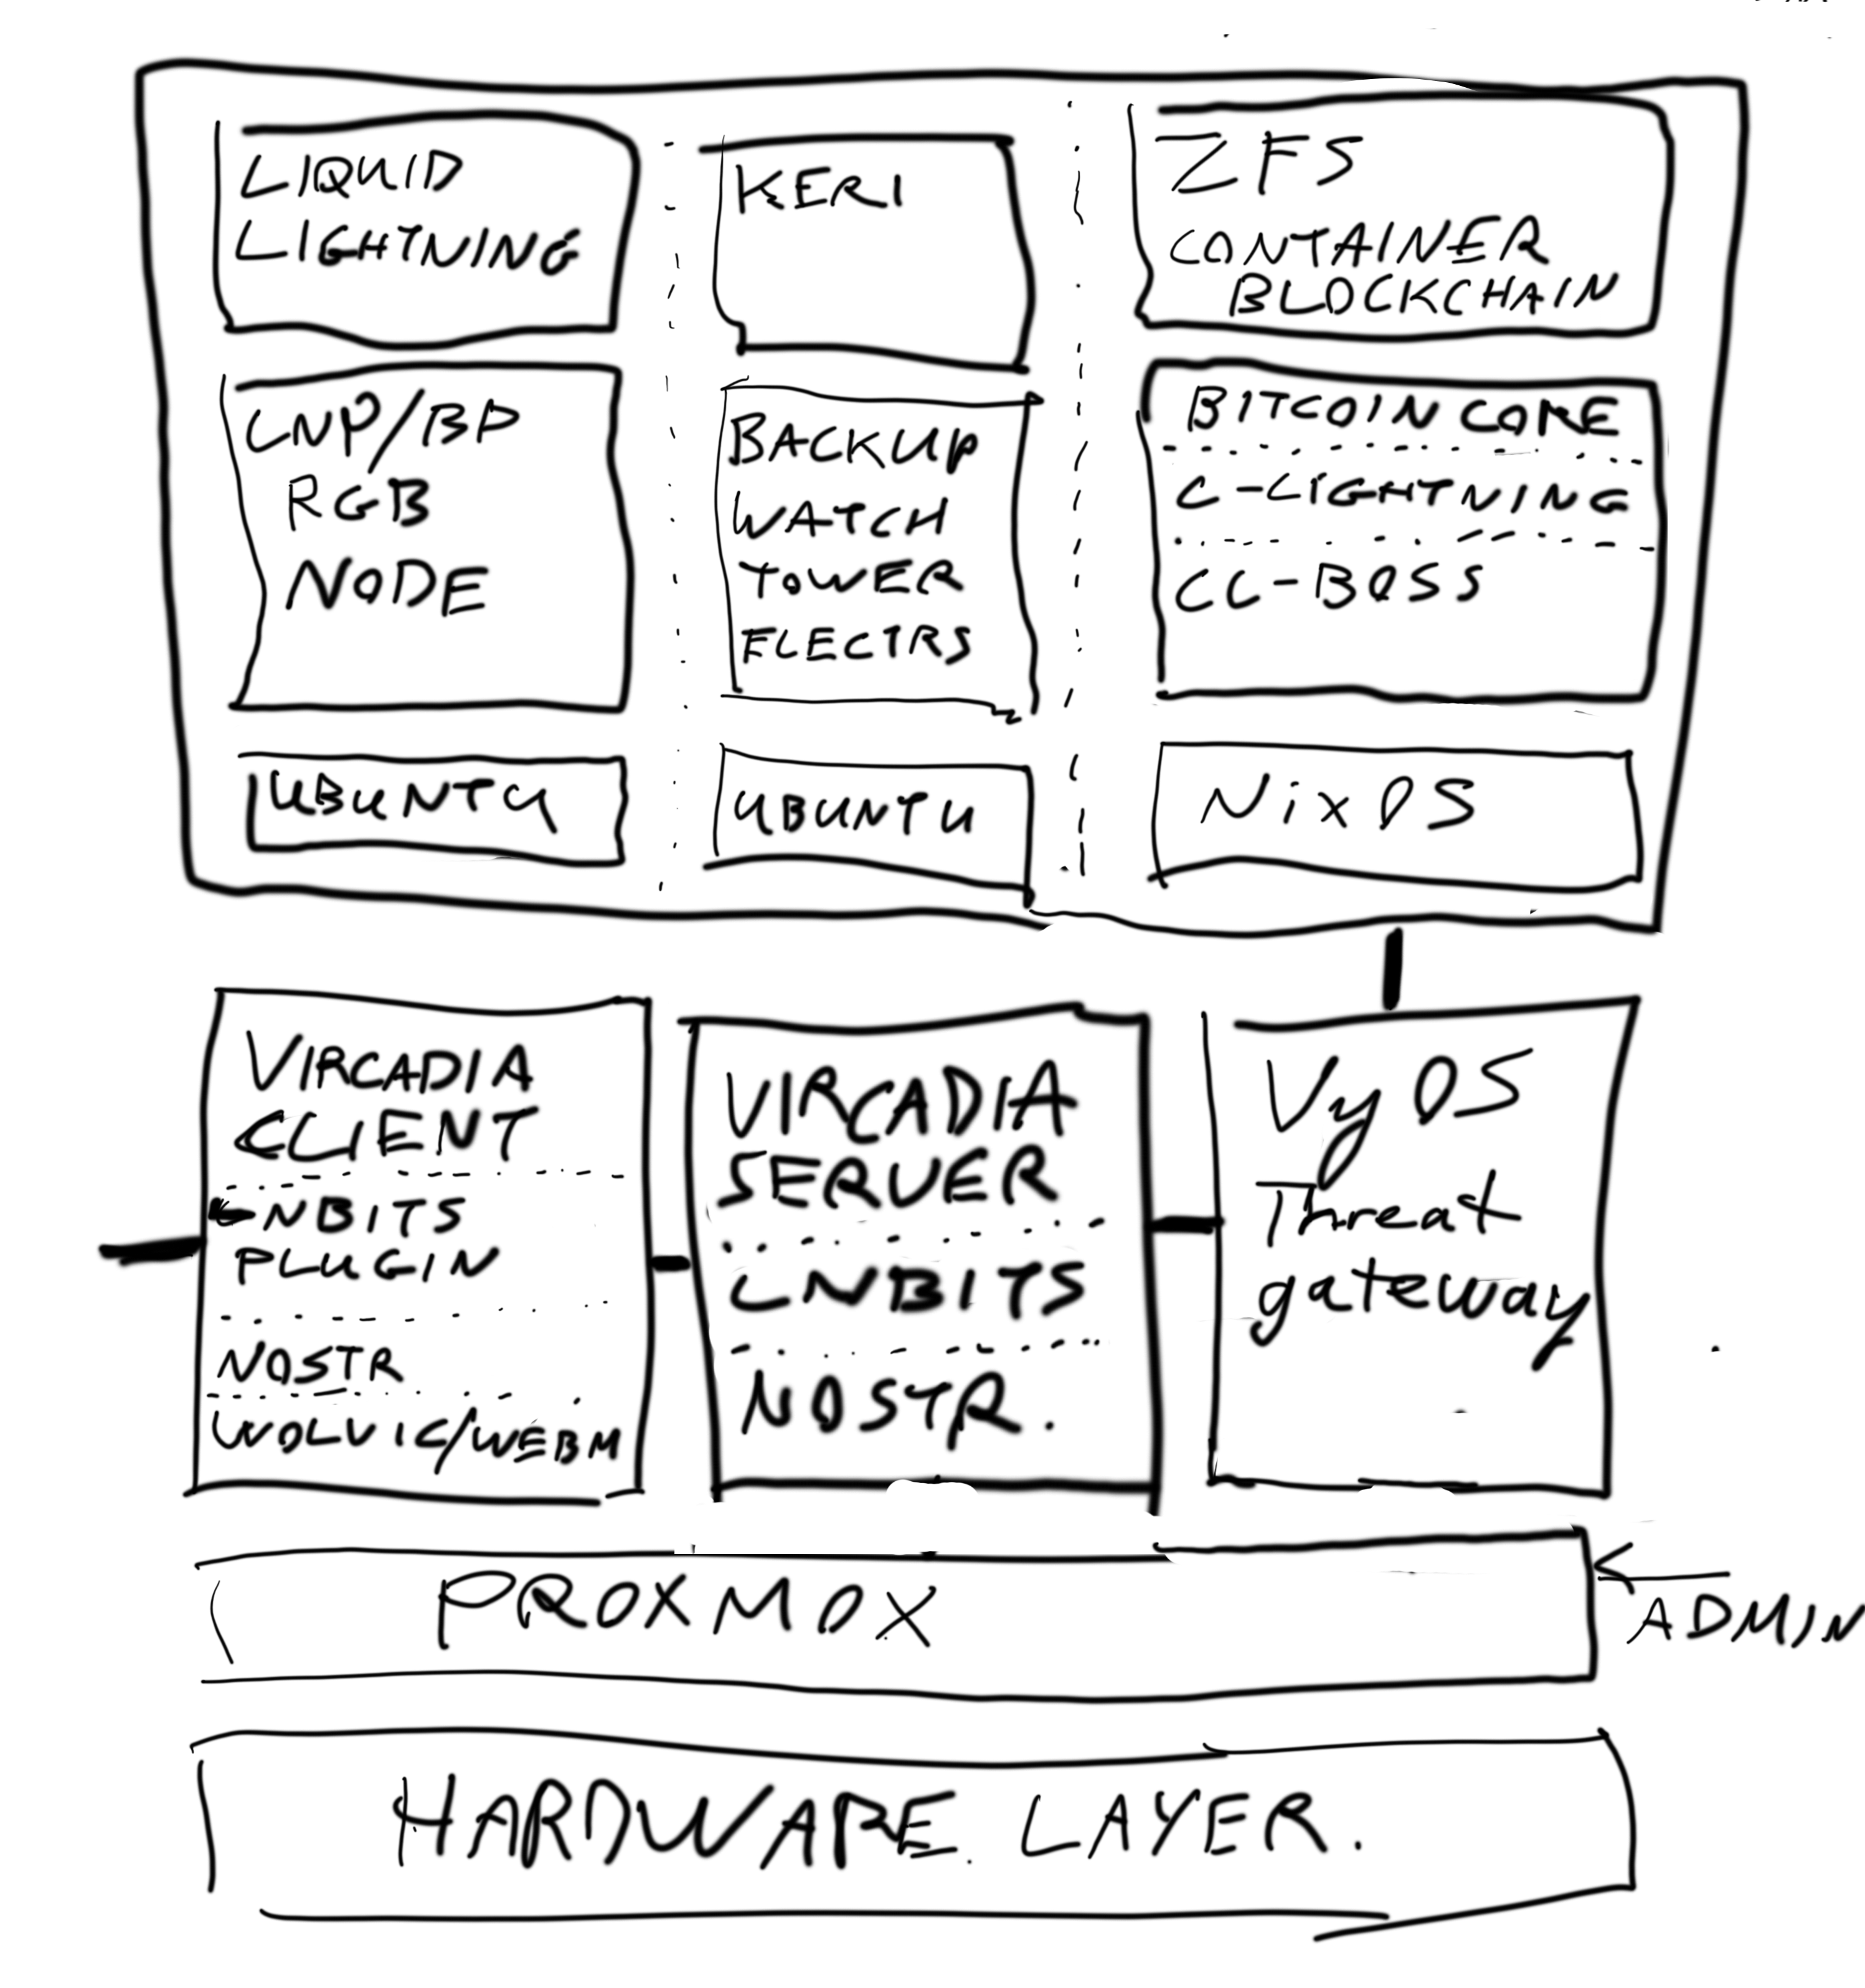
\includegraphics[width=\linewidth]{deployment}
	\caption{Proposed deployment of the software within the VMs on a single hardware system.}
	\label{fig:deployment}
\end{figure*}

\section{Networking layer}
\lipsum[50]
\subsection{Proxmox}
Proxmox open source server virtualisation allows the deployment of several virtual machines within a hardware system. Each of these VMs can have a different balance of performance, ease of use, and security. The VMs are given only the access they need to perform the task which they are specialised for. This improves overall security. Resilience is improved since elements of the cluster can be shutdown, reinstanced, and upgraded, without impacting the whole. Snapshots and backups are simplified.
\subsection{VyOS firewall}
VyOS firewall is a Proxmox aware threat management gateway and firewall which allows more nuanced interfacing with corporate systems, while maximising the security of the VM network which sits behind it i the virtual cluster.
\subsection{Privacy aspects and using TOR etc}
Currently some compromises with privacy may be necessary. Power users vs standard users. KYC/AML. 
\href{https://bitnodes.io/nodes/?q=.onion}{tor nodes}
\section{Bitcoin on Nix}
\lipsum[50]
\subsection{Bitcoin Core}
\lipsum[50]
\subsection{Electrum server}
\href{https://blog.blockstream.com/en-esplora-and-other-alternatives-to-electrumx/}{Options on the Blockstream website}
\lipsum[50]
\subsection{Lighting LND and LNBits}
\href{https://github.com/itsneski/lightning-jet}{Lightning Jet} automatic rebalance.
\subsection{C-Lightning and CLBoss}
\lipsum[50]
\subsection{Backup \& Watchtower}
\lipsum[50]
\subsection{RGB}
\lipsum[50]
\section{Liquid sidechain and Lightning (NFT enabled)}
\lipsum[50]

%About Lightning Tokens: 
%https://www.youtube.com/watch?v=4k6Im5yfum0

%Detailed interview about Slashtags and %Web 3.0 aspects:
%https://twitter.com/Synonym_to/status/1481514375194292225?s=20

%Overview on all products:
%https://www.youtube.com/watch?v=5Btf_OD_3pY

%This tweetstorm is our original presentation slides:
%https://twitter.com/Synonym_to/status/1460781350441689091?s=20

%Video of the presentation:
%https://bitcointv.com/w/p1dgZcEmQQiADixvx9MoE1
\lipsum[50]
\section{Identity}
\subsection{nostr}
\lipsum[50]
\subsection{KERI}
\lipsum[50]
\section{Metaverse}
\lipsum[50]
\subsection{Vircadia}
\lipsum[50]
\subsection{Wolvic}
``The goal of the Wolvic project is to create a full-featured browser exclusively for standalone AR and VR headsets.''\\
Wolvic is a continuation of the now defunct Firefox Reality Browser project. It is open source.
\subsection{WebM}
\href{https://www.webmproject.org/about/}{Free open source web video player}	
\lipsum[50]
\section{Messengers}
Matrix, NOSTR, Juggernaut
\chapter{Example deployment }
\lipsum[50]
\section{GitHub }
\lipsum[50]